\chapter{Methodolodgy}
\label{cha:Methodology}

%---------------------------------------------------------------------------
\section{Programming Environment}
\label{sec:programmingEnv}
Machine learning and data analysis projects are often executed using Jupyter notebooks. This study also utilized them due to their compatibility with Python, a language with extensive neural network training and result visualization libraries. Jupyter Notebooks seamlessly integrate Python code with explanatory comments and visualizations, facilitating well-documented work. The primary reason for selecting Jupyter Notebooks was their compatibility with Google Colab and Kaggle Notebooks, which provide free GPU resources. Utilizing GPUs significantly reduced network training time, enabling the evaluation of a much larger array of architectures and scenarios.

As previously mentioned, the technical part of the master thesis was conducted using the \textit{Python} programming language. Diagram \ref{fig:pythonLibraries} illustrates the libraries used. The specific versions of the libraries are included in the code.

\begin{figure}[!htb]
    \centering
    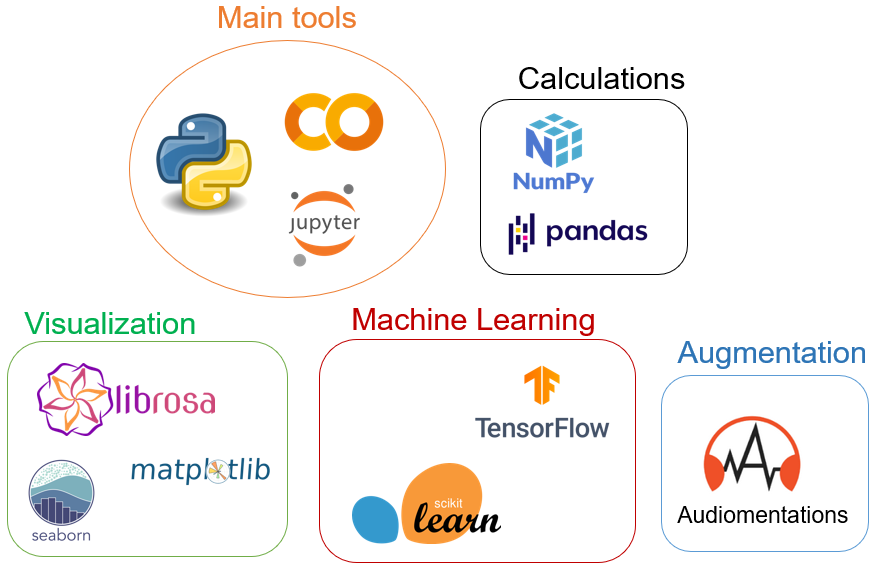
\includegraphics[scale=0.55]{Images/python-libraries.png}
    \caption{Programming language and libraries used in this thesis.}
    \label{fig:pythonLibraries}
\end{figure}

\section{Description of Datasets}
\label{sec:datasets}

To compare augmentation methods, various datasets were used to ensure more generalizable results. One dataset was selected for its typical and general characteristics, serving as a baseline. Another dataset was designed for one-shot learning, containing minimal data per class. The third dataset evaluated image augmentation in a domain-specific application, using audio files that are treated similarly to images.

%---------------------------------------------------------------------------

\subsection{Flowers 102 Dataset}
\label{ssec:Flowers102Dataset}

The Flowers $102$ dataset~\cite{Flowers102} consists of $8,189$ images, each depicting one of 102 different flower categories commonly found in the United Kingdom. Each category corresponds to a single species such as daisies, tulips, roses, and many others. The number of images per class varies, but each class is represented with at least $40$ images, which helps in training robust models.

\begin{figure}[!htb]
    \centering
    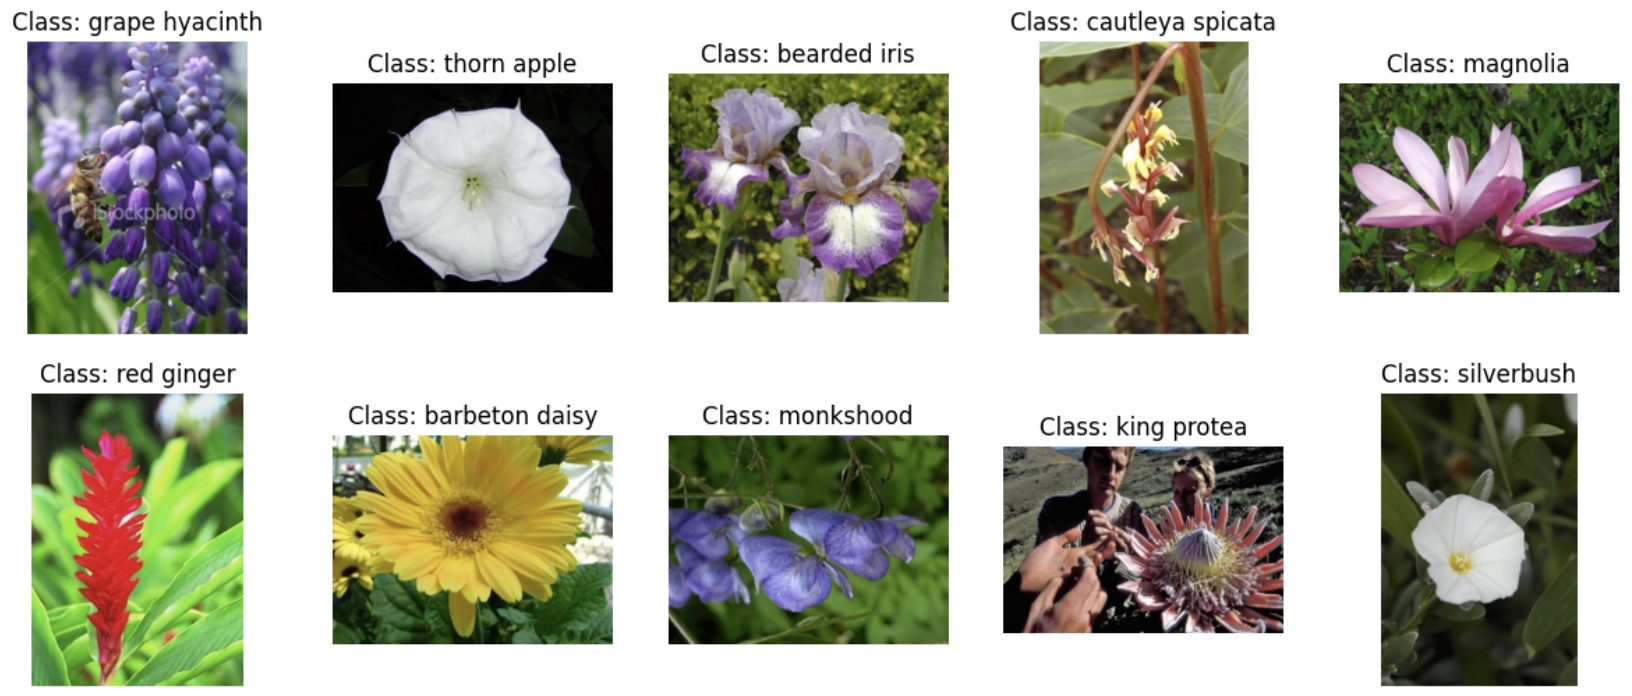
\includegraphics[scale=0.7]{Images/flowers-example.png}
    \caption{Samples from Flowers 102 dataset.}
    \label{fig:flowersExample}
\end{figure}

The Flowers 102 dataset is widely utilized for training and evaluating deep-learning models that specialize in image classification. Such models require exceptional recognition capabilities to distinguish between closely related species of flowers. As a standard dataset, it is highly respected in academic research for testing novel approaches in computer vision, machine learning, and especially in transfer learning, where pre-trained models are adapted to this dataset to achieve superior specificity. The dataset is frequently referenced in research papers and leveraged in diverse machine-learning competitions and educational initiatives to evaluate algorithm effectiveness.

One key challenge the Flowers 102 dataset poses is the intra-class variation and inter-class similarity. Some flower species in the dataset have considerable variation in appearance due to different growth conditions and developmental stages, while different species may look quite similar to each other. Shape isomap is shown in Figure \ref{fig:shapeIsomap}.

\begin{figure}[!htb]
    \centering
    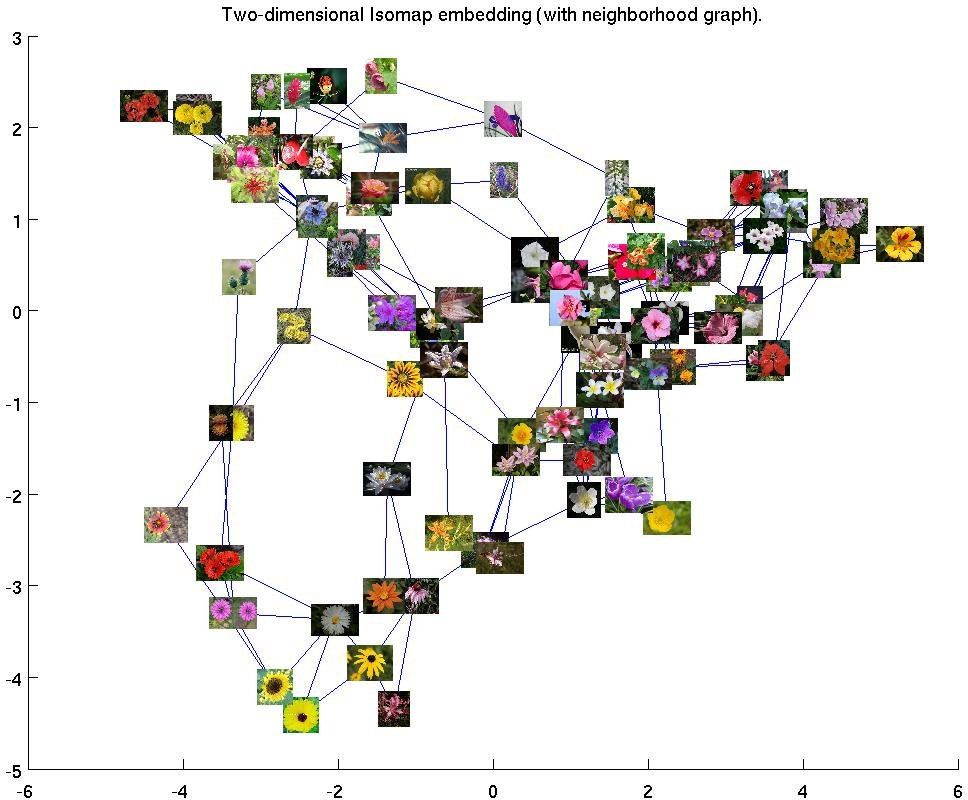
\includegraphics[scale=0.3]{Images/shape-iso.jpg}
    \caption{Shape isomap of Flowers 102 dataset~\cite{Flowers102}.}
    \label{fig:shapeIsomap}
\end{figure}

%---------------------------------------------------------------------------

\subsection{One-shot Flowers 102 Dataset}
\label{ssec:flowersOneShotDataset}

To tackle the difficulties of one-shot learning, smaller datasets were created based on "Flowers 102"~\cite{Flowers102}. Specifically, \textbf{5, 10 or 20 images were selected at random from each of the 102 flower categories} to investigate the efficiency of data augmentation techniques under these conditions. With a limited number of images per class, the risk of overfitting and the need for the model to generalize from a small set of examples are significant challenges. However, by implementing data augmentation techniques, it should be possible to improve the model's performance significantly. 



%---------------------------------------------------------------------------

\subsection{GTZAN Dataset}
\label{ssec:gtzanDataset}

The GTZAN dataset~\cite{GTZAN} is one of the pioneering collections for music genre classification, comprising a total of 1,000 audio tracks each lasting 30 seconds. The dataset is evenly distributed across 10~different genres, including blues, classical, country, disco, hip-hop, jazz, metal, pop, reggae, and rock, with each genre represented by 100 tracks. This uniform distribution aids in creating balanced classification models.

\begin{figure}[!htb]
    \centering
    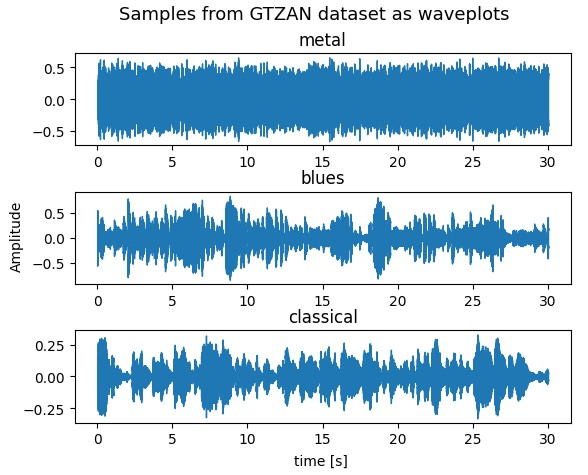
\includegraphics[scale=0.6]{Images/gtzan-example.jpg}
    \caption{Samples from GTZAN dataset~\cite{GTZAN} visualized as waveforms.}
    \label{fig:gtzanExample}
\end{figure}

Widely used in evaluating machine learning models for music analysis, the GTZAN dataset has become a benchmark in the field. It allows researchers to test and demonstrate the efficiency of various audio processing techniques and algorithms to understand and categorize musical styles. Models trained on the GTZAN dataset often employ techniques like Fourier transforms to capture frequency components and machine learning algorithms such as k-nearest neighbors, decision trees, and neural networks to classify audio samples.

In this research, the GTZAN dataset was utilized to explore the impact of data augmentation techniques on \textbf{domain-specific} data. Methods such as time stretching, pitch shifting, and adding background noise were implemented to investigate how these augmentations could enhance the robustness of genre classification models. The focus was on addressing overfitting and improving model generalizability across varied musical inputs.

A notable challenge when working with the GTZAN dataset involves handling the diversity within each genre and the potential overlap between different genres, where certain tracks might share characteristics typical of multiple genres. Another issue is the quality and encoding of the audio tracks, which can affect the performance and generalization capability of the trained models. Additionally, to utilize this dataset with traditional image classification methods, it is necessary to convert the data into MEL Spectrograms. 

In academic circles, the dataset is frequently cited for illustrating the capabilities and limitations of computational approaches to music genre recognition. This is another reason why this dataset was chosen.

%---------------------------------------------------------------------------

\section{Data Preprocessing and Augmentation}

\subsection{Steps common for all datasets}
\label{ssec:commonProcessing}

The initial datasets were loaded and categorized following the existing directory structure to ensure \textbf{consistent data organization}. This systematic arrangement allowed for an intuitive mapping between the data categories and their respective labels.

A \textbf{seed} was set at the beginning of the process for \textbf{NumPy}, \textbf{TensorFlow}, and the \textbf{random} package to ensure repeatability across multiple experimental runs. This is crucial for accurate reproduction and comparison of results, which is essential when evaluating the efficacy of various models and experiments.

Subsequently, the data was divided into \textbf{training, validation, and test sets} in approximate proportions of 70\%, 20\%, and 10\%, respectively. The split was chosen to facilitate optimal training of neural networks while maintaining an adequate validation and testing set. The division was stratified, which means that it was arranged in a way that ensures an even distribution of classes in all sets. Cross-validation was not utilized due to the significant computational time required for training neural networks in each fold.


The \textbf{labels were encoded using one-hot encoding} to facilitate their use in training neural networks. This encoding method transforms categorical labels into a binary matrix, where each column corresponds to a unique class. One-hot encoding ensures compatibility with the network's output layer and simplifies the representation of categorical data. Additionally, this encoding approach enables the application of data augmentation techniques such as \textit{MixUp} and \textit{CutMix}.

The images were then grouped into \textbf{batches} containing 32 examples each to streamline the training process. The number of \textbf{epochs} was carefully chosen to balance training time and model performance, ensuring that the networks had sufficient time to learn from the data without overfitting.

Regarding data augmentation, it could be \textbf{turned on or off} for each experiment to assess its impact. The \textbf{probability of augmentation} occurring was configurable separately for traditional techniques, \textit{MixUp}, \textit{CutMix}, and others, allowing fine-tuning of the augmentation process for the specific characteristics of each problem. This flexibility ensured that the augmentation strategy was optimized to address the challenges of the dataset and improve model performance accordingly.

\textbf{TensorFlow datasets} which defined processing and augmentation steps were built for each dataset used in the experiments. As the preprocessing and dataset preparation varied between datasets, the specific details for each will be described separately in the following sections.

\subsection{Flowers 102}
\label{ssec:Flowers102Processing}

In the processing and augmenting of the Flowers 102 dataset, a series of steps were implemented to strengthen the training data. The images were \textbf{flipped horizontally} to mimic the natural left-right growth patterns of flowers, while \textbf{brightness} and \textbf{contrast} modifications simulated the diverse lighting environments existing in nature. A \textbf{Gaussian filter} was utilized to replicate natural blurring and noise.

The images were \textbf{rotated up to 45 degrees} in either direction, as flowers typically do not grow at extreme angles. The noise was injected to reflect environmental disturbances and camera sensor noise. \textbf{Random cropping} was applied to emulate zooming, which helped the model identify flowers from varying distances.

The process of augmentation was carried out based on the probabilities mentioned in the previous section. After these adjustments, all images were \textbf{resized to 224 x 224 pixels} to comply with the standard input dimensions of \textit{ResNet} and \textit{EfficientNet}. \textit{MixUp} and \textit{CutMix} were also used across batches to enrich the dataset and boost the model's generalization capacity.

\begin{figure}[!htb]
    \centering
    \begin{subfigure}{0.7\textwidth}
        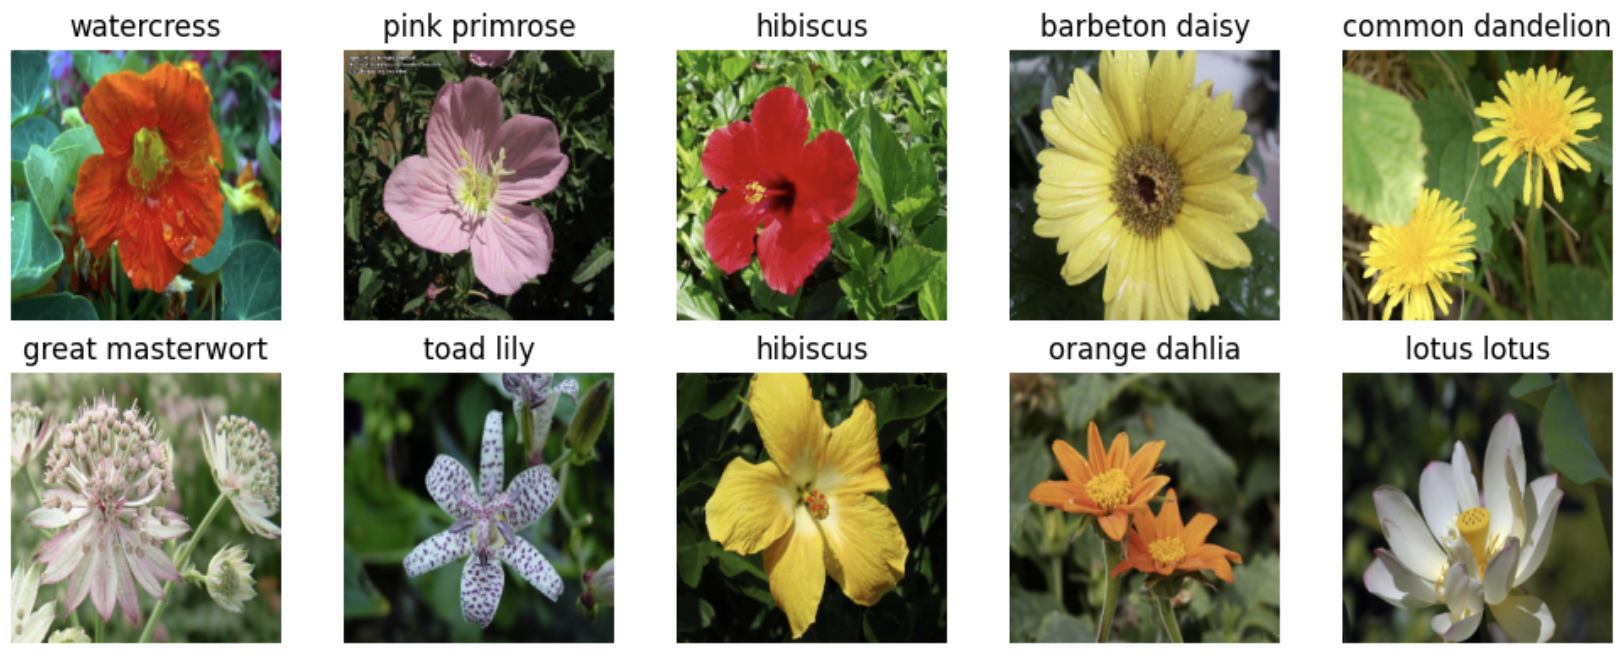
\includegraphics[scale=0.50]{Images/no-augmentation.png}
        \caption{No Augmentation}
    \end{subfigure}
    \vspace{0.3cm}

    \begin{subfigure}{0.7\textwidth}
        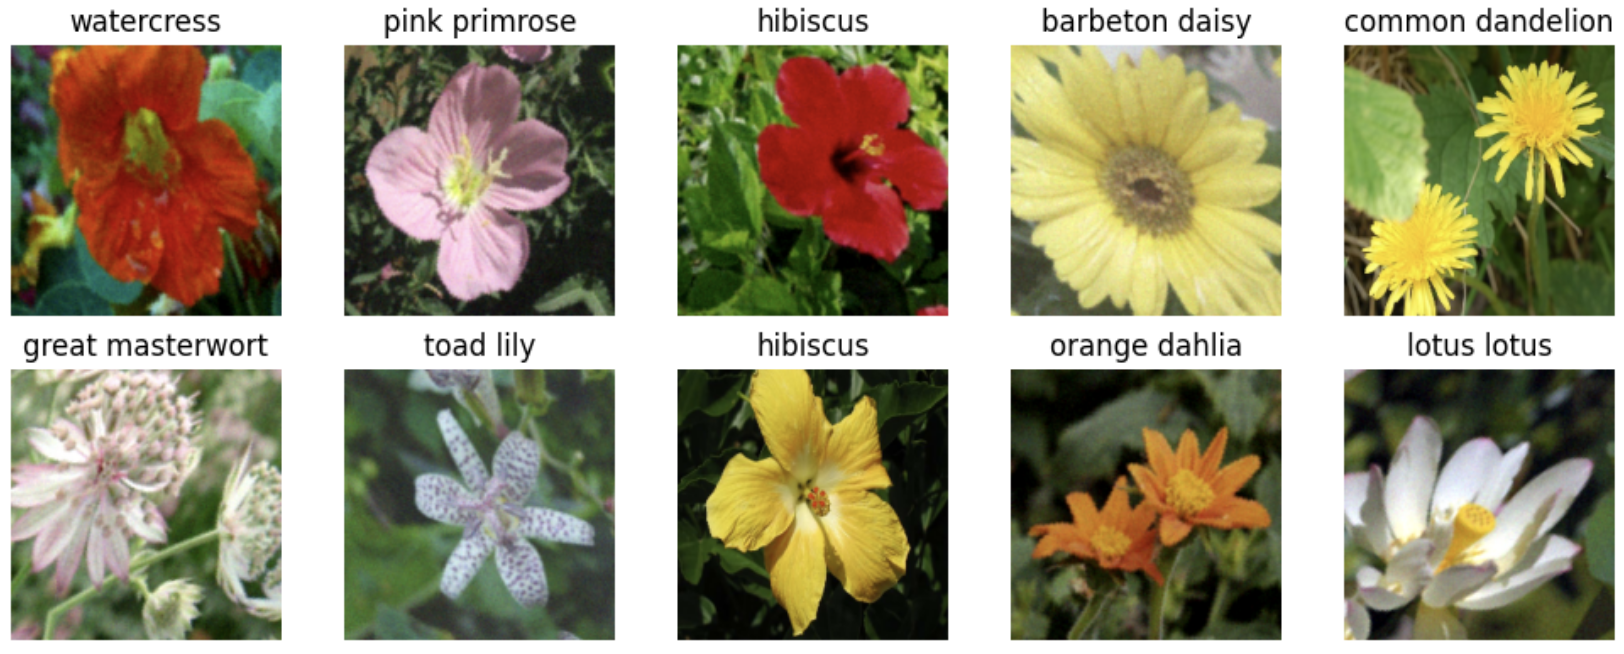
\includegraphics[scale=0.50]{Images/traditional-augmentation-4.png}
        \caption{Traditional Augmentation}
    \end{subfigure}
    \vspace{0.3cm}

    \begin{subfigure}{0.7\textwidth}
        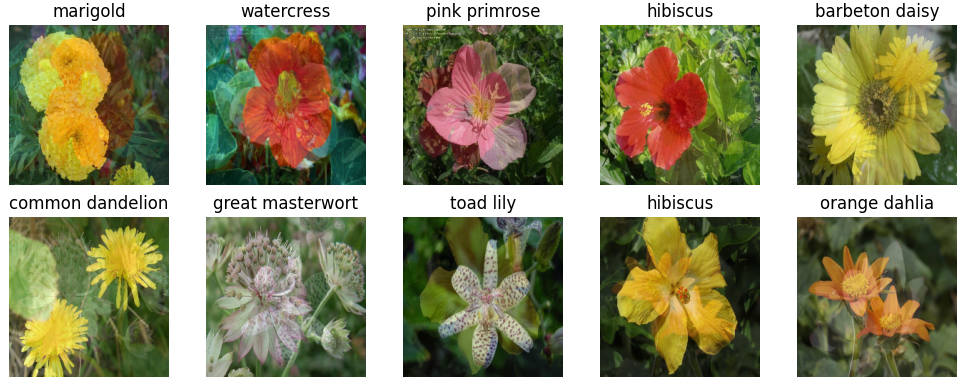
\includegraphics[scale=0.85]{mixup-augmentation.png}
        \caption{\textit{MixUp} Augmentation}
    \end{subfigure}
    \vspace{0.3cm}

    \begin{subfigure}{0.7\textwidth}
        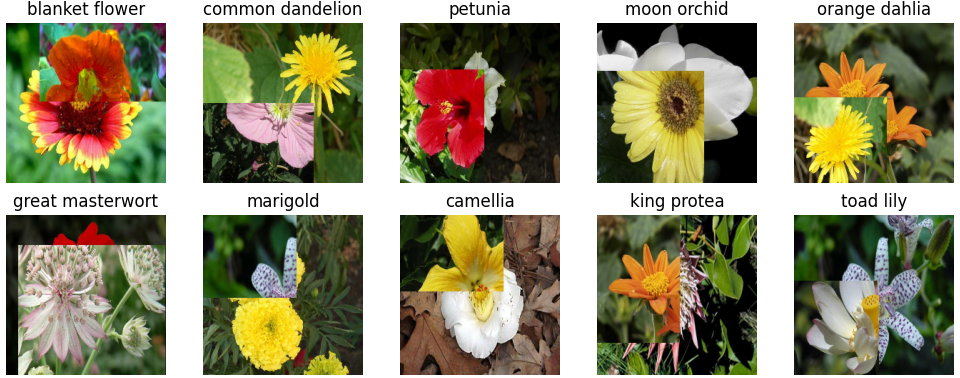
\includegraphics[scale=0.85]{cutmix-augmentation.png}
        \caption{\textit{CutMix} Augmentation}
    \end{subfigure}

    \caption{Augmentations applied to Flowers 102 and One-shot Flowers 102 Datasets. (Source: a) \cite{Flowers102}, b-d) the images augmented with own implementation.)}
    \label{fig:flowersAugmentations}
\end{figure}

As illustrated in Figure \ref{fig:flowersAugmentations}, multiple augmentations can occur simultaneously. For instance, in the image (b), the \textit{Barbeton daisy} flower was rotated, zoomed, and adjusted for contrast at the same time. However, \textit{Hibiscus} flower was not changed at all. It ensures that in each epoch different images are affected and variability of data achieved by augmentation is higher. 

In image (c) we can see \textit{MixUp} augmentation, which impacts both images and labels. For instance, if 30\% of the first image and 70\% of the second image are combined, their corresponding one-hot encoded values will be adjusted to 0.3 and 0.7, respectively. Similarly, in image (d), the \textit{CutMix} augmentation modifies the image and labels based on the visible area. These augmentations can also be combined concurrently, enabling higher data variability and model generalization.

\subsection{One-shot Flowers 102}
\label{ssec:flowersOneShotProcessing}

Processing steps were the same as those described in the previous section except that at the beginning, as mentioned in section \ref{ssec:Flowers102Dataset}, the number of data samples per category was \textbf{restricted to 5, 10, and 20} to explore data augmentation effectiveness in a setting with limited data. The number of epochs was adjusted -- for a smaller amount of examples, more epochs were needed to learn valuable features for validation data classification. If the number of examples in the original dataset was smaller than the restriction threshold, examples were randomly repeated for some classes. 

Since the goal was to train the model under conditions with limited data,  the \textbf{validation set} was extracted from the training set, further reducing the number of training cases below the desired threshold. The \textbf{test set} remained unchanged from the full Flowers 102 dataset to ensure a valid comparison.

\subsection{GTZAN}
\label{ssec:gtzanProcessing}

In addition to the general techniques outlined in section \ref{ssec:commonProcessing}, specific steps were applied to the GTZAN dataset for image augmentation. The original files in the dataset, which have a \textbf{*.wav extension}, required transformation into a format suitable for visual processing. To achieve this, audio files were converted into Mel Spectrograms. Figure \ref{fig:waveSpecExample} shows an illustrative example of the classical music data before and after the transformation from a wave into spectrogram form.

\begin{figure}[!htb]
    \centering
    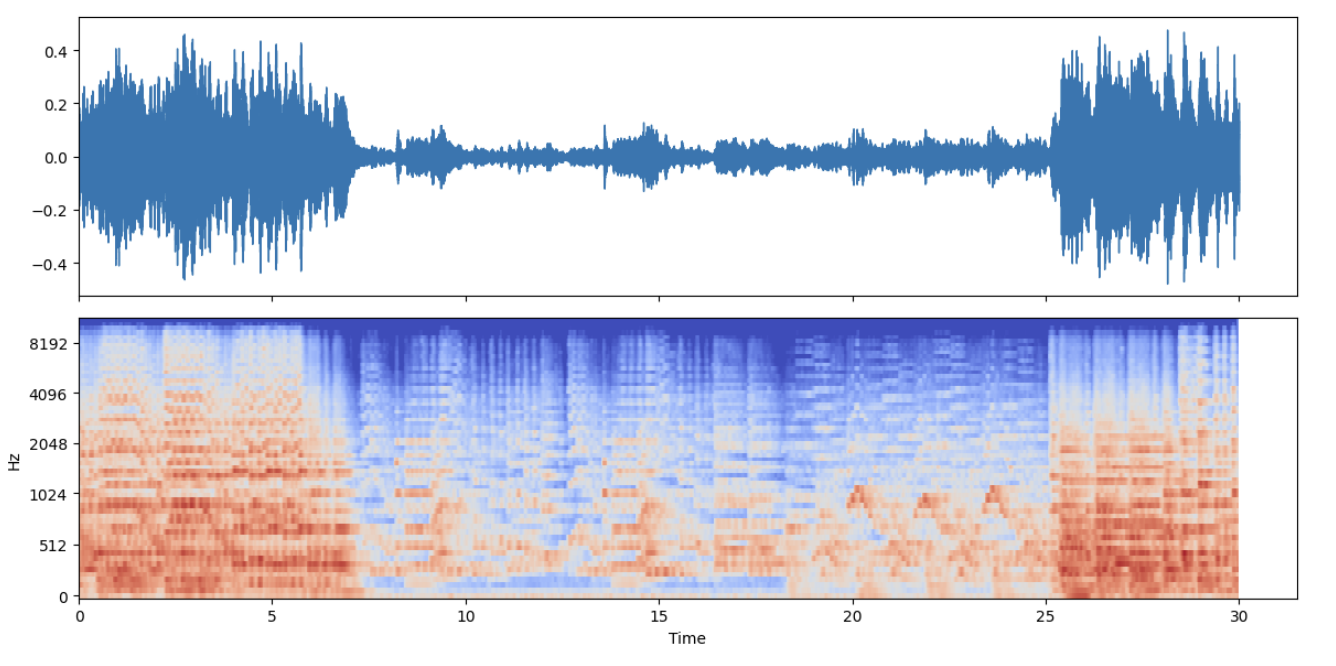
\includegraphics[scale=0.7]{Images/wave-spec-classical.png}
    \caption{Waveform and Spectrogram of classical music. Source:~\cite{GTZAN}.}
    \label{fig:waveSpecExample}
\end{figure}

Parameters of the Short-Time Fourier Transform (STFT) used for this transformation are detailed in the Table \ref{tab:parameters}.
These parameters were chosen based on the literature as detailed in~\cite{GTZANParameters}. The transformation process, implemented in Python's Librosa library, was essential for visualizing and augmenting the data within the framework of image processing techniques, which is the main focus of this thesis.

\begin{table}[h!]
\centering
\caption{Mel Spectrogram parameters.}
\begin{tabular}{|>{}l|l|}
\hline
\textbf{Parameters}    & \textbf{Values}  \\ \hline
Window size            & 1024    \\ \hline
Hop length             & 512     \\ \hline
Number of FFT points   & 4096    \\ \hline
Number of MEL bands    & 64      \\ \hline
Minimum frequency      & 0 Hz    \\ \hline
Maximum frequency      & 8000 Hz \\ \hline
Normalization          & True    \\ \hline
\end{tabular}
\label{tab:parameters}
\end{table}

Moreover, at the waveform level, cropping or padding was used to standardize the length of all audio files before feeding them into the network. Additionally, time shifting and stretching, pitch shifting, and Gaussian noise were incorporated to enhance variability in the training data.

Time and frequency masking were applied after the waveforms were converted into spectrograms. The number and width of the masked strips were adjustable. Furthermore, \textit{MixUp} was applied to the spectrograms using a similar approach as described in previous sections. During training, all types of augmentation were randomly combined using independent probabilities of occurrence. All augmentation types applied to the GTZAN dataset are visualized in Figure \ref{fig:GTZANAugmentations}.

\begin{figure}[!htb]
    \centering
    \begin{subfigure}{0.9\textwidth}
        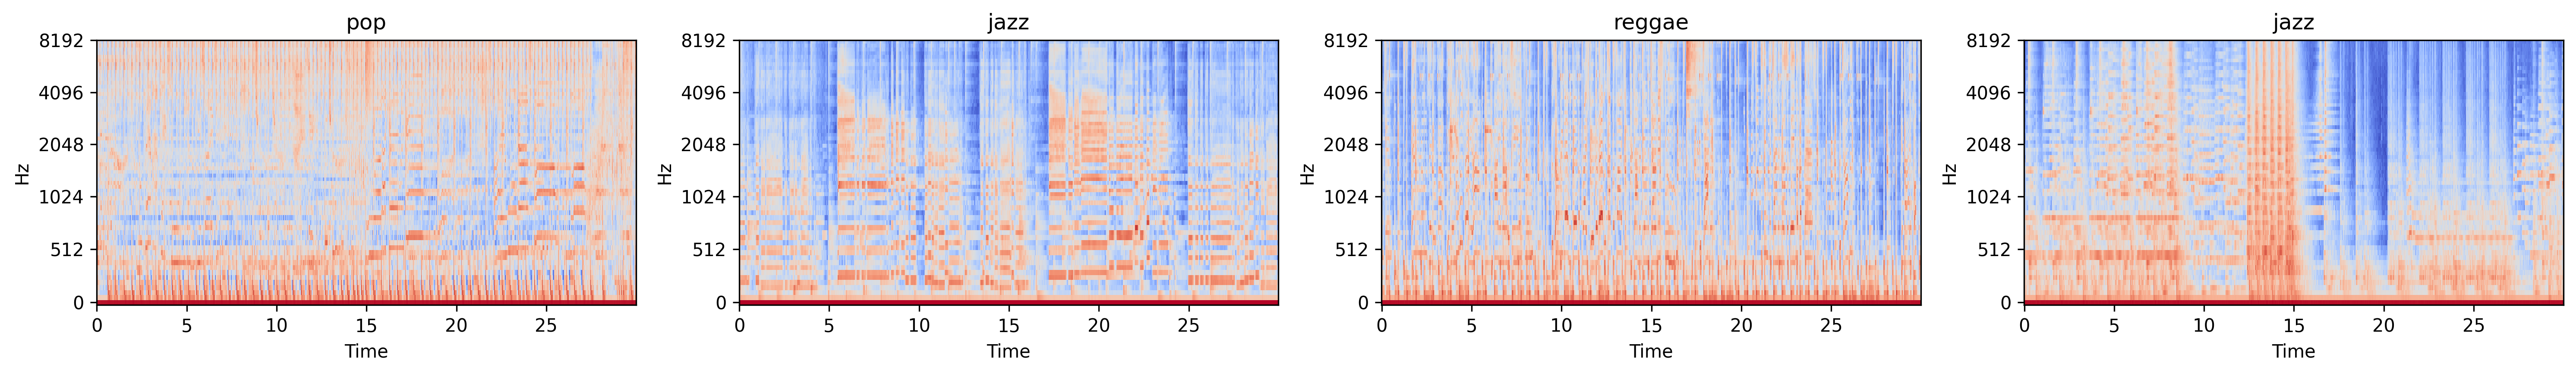
\includegraphics[scale=0.28]{Images/gtzan_new/no_augmentation.png}
        \caption{No Augmentation}
    \end{subfigure}
    \vspace{0.3cm}

    \begin{subfigure}{0.9\textwidth}
        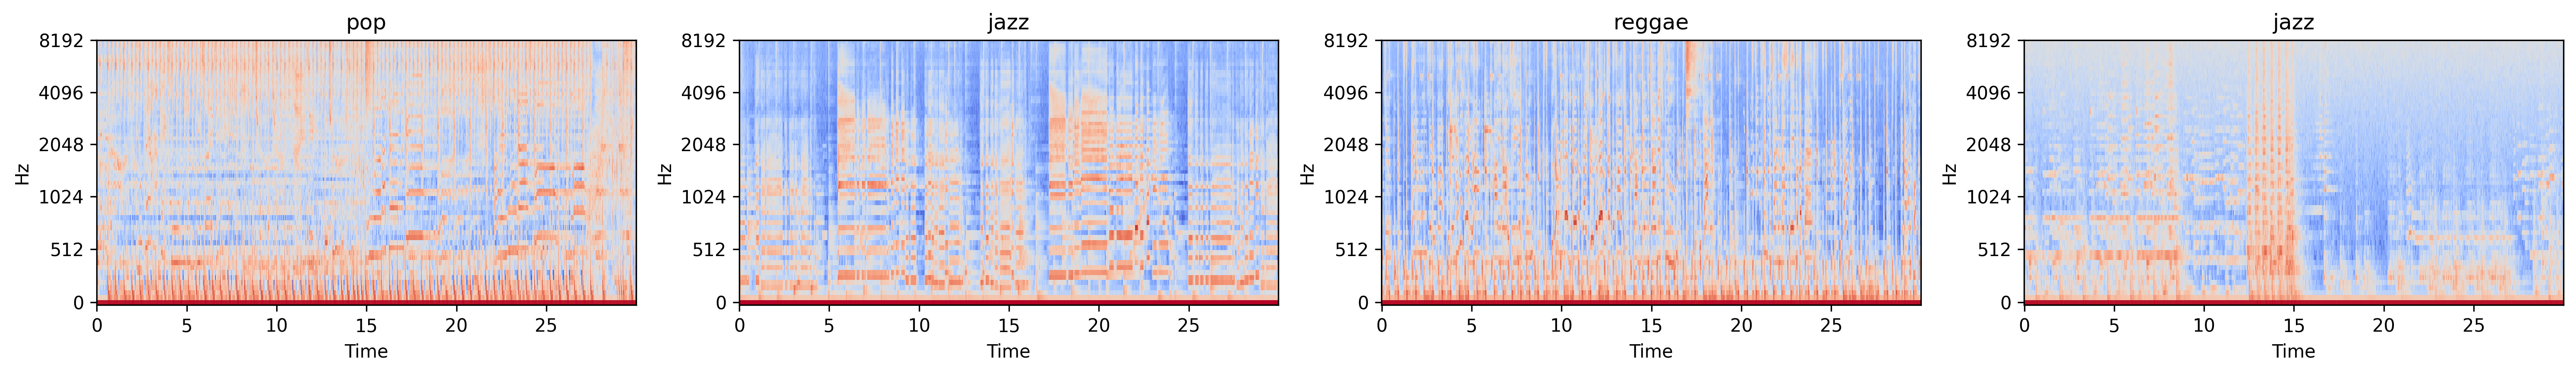
\includegraphics[scale=0.28]{Images/gtzan_new/gn_augmentation.png}\
        \caption{Gaussian Noise}
    \end{subfigure}
    \vspace{0.3cm}

    \begin{subfigure}{0.9\textwidth}
        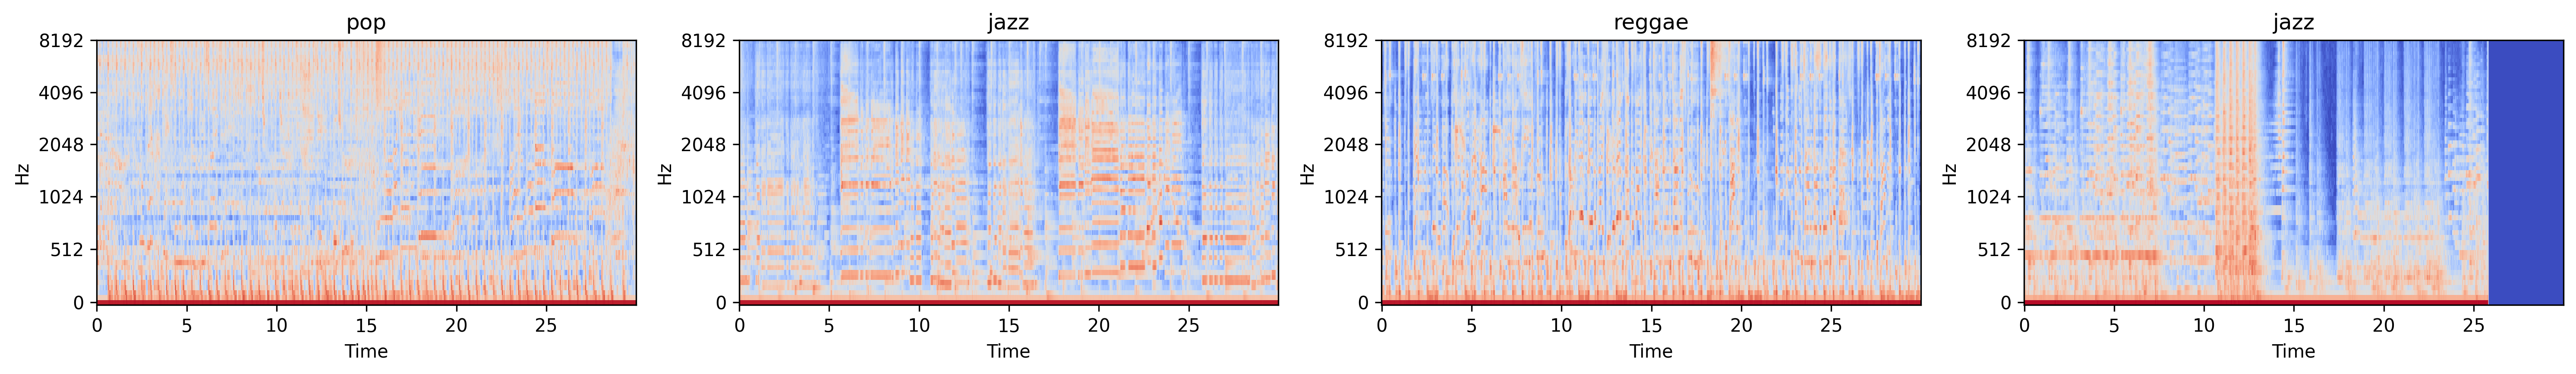
\includegraphics[scale=0.28]{Images/gtzan_new/speedchange_augmentation.png}
        \caption{Speed Change}
    \end{subfigure}
    \vspace{0.3cm}

    \begin{subfigure}{0.9\textwidth}
        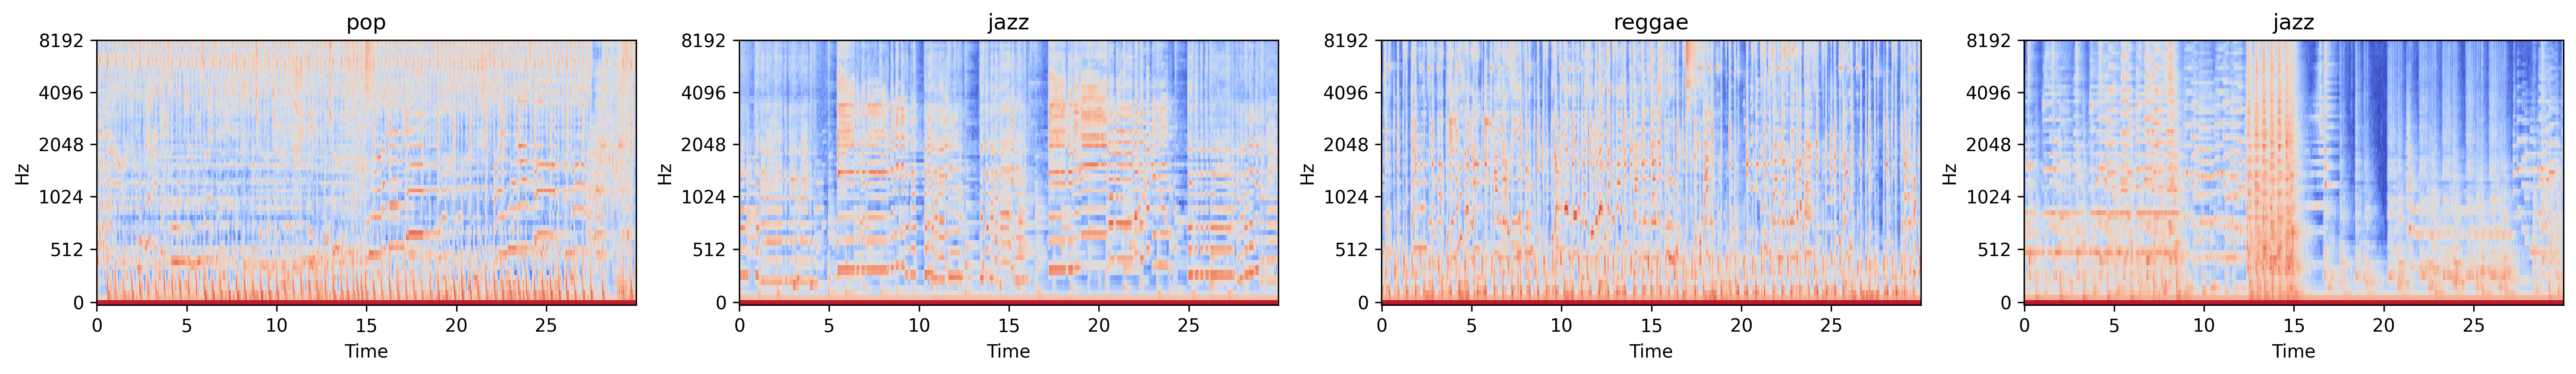
\includegraphics[scale=0.28]{Images/gtzan_new/pitchshift_augmentation.png}
        \caption{Pitch Shift}
    \end{subfigure}

    \begin{subfigure}{0.9\textwidth}
        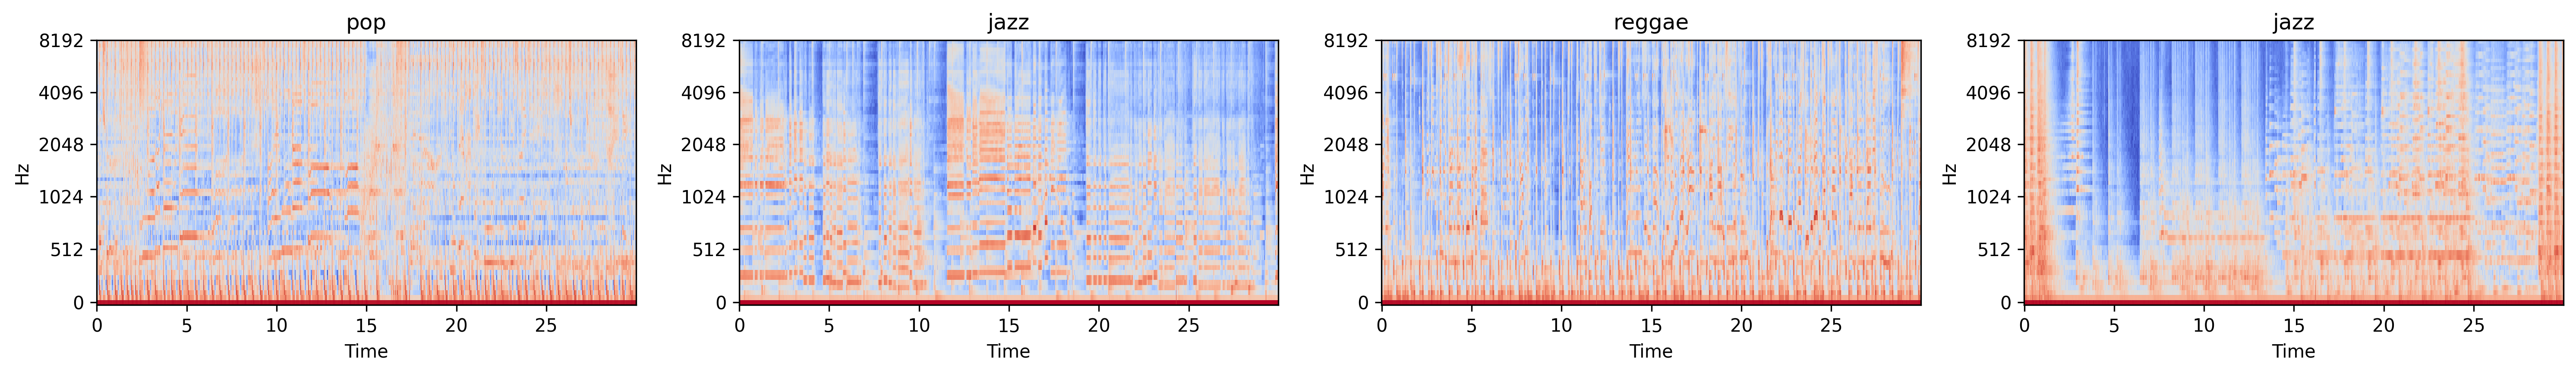
\includegraphics[scale=0.28]{Images/gtzan_new/time_shift_augmentation.png}
        \caption{Time Shift}
    \end{subfigure}

    \begin{subfigure}{0.9\textwidth}
        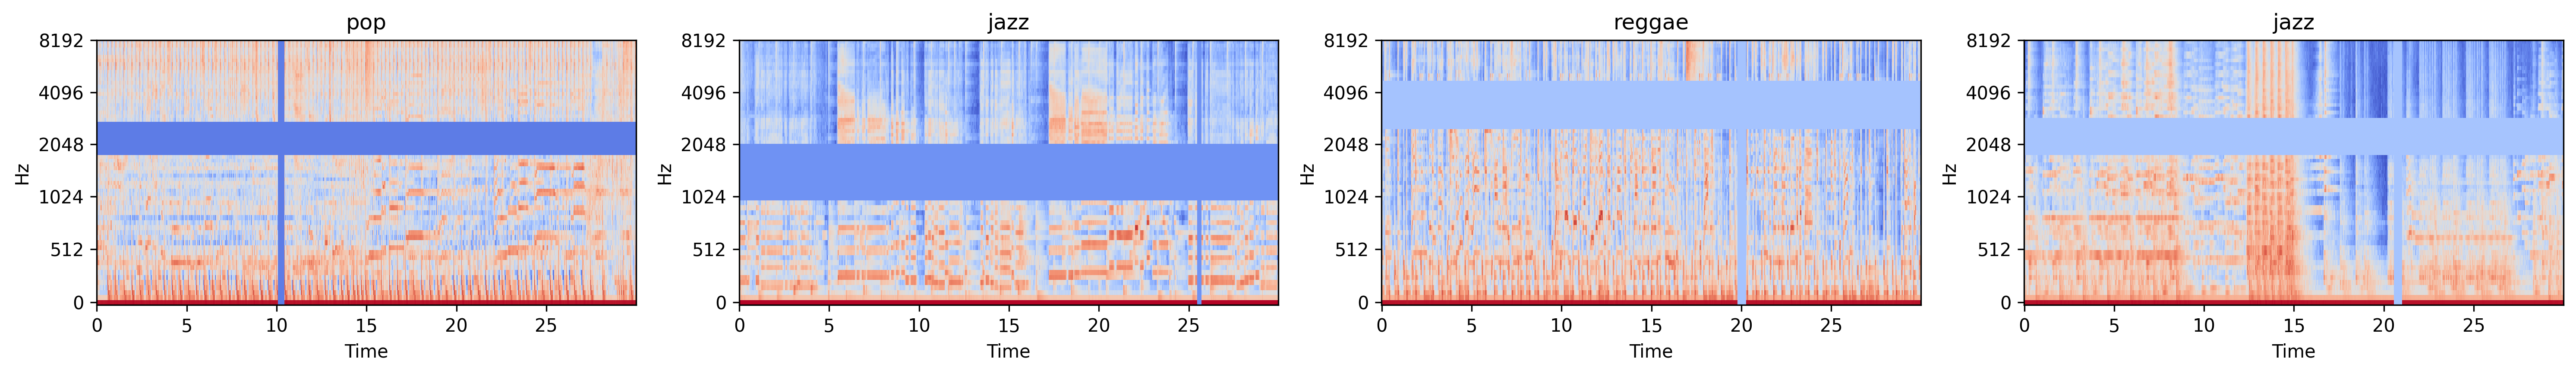
\includegraphics[scale=0.28]{Images/gtzan_new/masking_augmentation.png}
        \caption{Masking Augmentation}
    \end{subfigure}

    \begin{subfigure}{0.9\textwidth}
        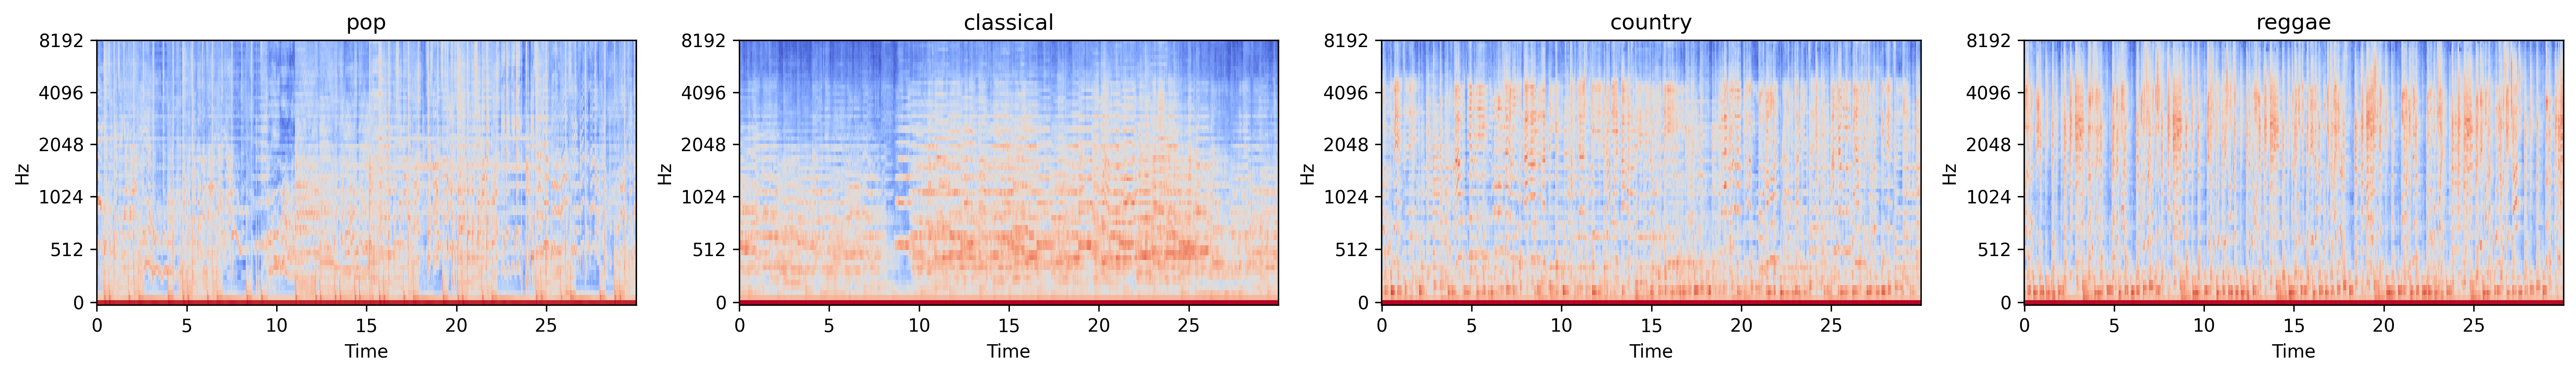
\includegraphics[scale=0.28]{Images/gtzan_mixup_augmentation.png}
        \caption{\textit{MixUp} Augmentation}
    \end{subfigure}

    \caption{Augmentations applied to GTZAN Dataset. Source: a) \cite{GTZAN}, b-g) the images augmented with own implementation.}
    \label{fig:GTZANAugmentations}
\end{figure}



%---------------------------------------------------------------------------

\section{CNN Architectures Used}

In this section, the model architectures used in the experiments are described, specifically \textit{ResNet50}, \textit{EfficientNetB0}, and \textit{EfficientNetB4}. Each model was constructed with appropriate modifications to suit the task, leveraging the principles of transfer learning discussed in previous chapters.

\textbf{ResNet50:} For the ResNet50 model, the base architecture was loaded without the top classification layers using pre-trained weights from ImageNet. All layers were set to trainable to enable fine-tuning. Custom layers were added on top of the base model, including a Global Average Pooling layer followed by a Dense layer with a softmax activation function for classification. The model was then compiled with an appropriate optimizer, loss function, and evaluation metrics.

\textbf{EfficientNetB0, EfficientNetB4}:  The EfficientNet model followed a similar approach. The base EfficientNet architecture was loaded without the top layers, and pre-trained weights from ImageNet were utilized. An input layer was defined, and the base model was applied to this input. A Global Average Pooling layer was added, followed by a Dense layer with 32 neurons, batch normalization, and dropout for regularization. The final Dense layer used a softmax activation function for classification. The model was compiled with the necessary components for training.

In case of the GTZAN dataset, the input shape was $64 x 1292$, which is different from the default one. The number of parameters for each network is shown in Table \ref{tab:modelParameters}.
\begin{table}[h]
    \centering
    \caption{Comparison of Model Parameters.}
    \begin{tabular}{|c|c|c|}
        \hline
        \textbf{Model} & \textbf{All Parameters} & \textbf{Trainable Parameters} \\
        \hline
        ResNet50 & 23,608,202 & 23,555,082 \\
        \hline
        EfficientNetB0 & 4,091,021 & 4,091,021 \\
        \hline
        EfficientNetB4 & 17,731,657 & 17,606,386 \\
        \hline
    \end{tabular}
    \label{tab:modelParameters}
\end{table}


\section{Models Training}

In this section, the training process for the models using two datasets, Flowers 102 and GTZAN, is described.

The \textbf{Adam optimizer} was used for both datasets as it is a standard choice for neural networks due to its efficiency and adaptability. The loss function employed was Categorical Cross Entropy (CCE), appropriate for the multiclass classification problem at hand.

\textbf{Learning Rate:} For the Flowers 102 dataset, a learning rate of $1 \cdot 10^{-5}$ was chosen due to instability issues with higher learning rates, whereas for the GTZAN dataset, a learning rate of $1 \cdot 10^{-4}$ was utilized.

\textbf{Training Environment:} Training on the Flowers 102 dataset was conducted on a GPU and for the GTZAN dataset TPU accelerator was utilized. The decision was based on the GTZAN dataset's higher RAM requirements and the more powerful CPU capabilities of the TPU instances but also due to the availability of separate Kaggle notebooks free usage limits for GPUs and TPUs. 

\textbf{Data Splitting:} A standard train-validation-test split was used for both datasets, without cross-validation (CV). The reason for not using CV was the significant amount of time required to train the models.

\textbf{Batch Size} of $32$ was used for both datasets. Validation accuracy was \textbf{monitored} to choose the best model, which was not necessarily the last one trained. The model weights were saved at the end of each epoch. The number of epochs was equal to 50 for both the GTZAN dataset and the Flowers 102 dataset because the GTZAN dataset required similar iterations to stabilize.

\textbf{Logging:} training of each model was monitored and logged using the Weights and Biases (wandb) platform~\cite{wandb}. All the metrics detailed in Section \ref{sec:evaluationMetrics} were recorded, along with the model's weights and several additional custom visualizations.


%---------------------------------------------------------------------------

\section{Evaluation Metrics}
\label{sec:evaluationMetrics}

In this section of the thesis, performance evaluation metrics for classification are presented based on~\cite{ClassificationMetrics}. These metrics are specifically those employed for the evaluation in this study.

In image classification tasks, evaluating the performance of classifiers involves various metrics derived from the confusion matrix. The confusion matrix itself is a fundamental tool for understanding the classification results, especially in the context of accuracy, precision, recall, F1 score, and the confusion matrix itself. These metrics are described below.

\textbf{Confusion Matrix}: The confusion matrix for a multi-class classification problem is an $m$ x $m$ table, where $m$ is the number of classes in our dataset. Each row of the matrix represents the instances of an actual class, while each column represents the instances of a predicted class. For a class $i$, the following elements are crucial:
\begin{itemize}
    \item \textbf{True Positives ($TP_i$)}: The number of correctly predicted instances of class $i$.
    \item \textbf{False Negatives ($FN_i$)}: The number of instances of class $i$ that were incorrectly predicted as other classes.
    \item \textbf{False Positives ($FP_i$)}: The number of instances of other classes that were incorrectly predicted as class $i$.
    \item \textbf{True Negatives ($TN_i$)}: The number of instances that were correctly predicted as other classes, excluding class $i$.
\end{itemize}

Analyzing the confusion matrix helps us identify which classes are frequently misclassified as one another, providing insights into potential areas for model improvement. This analysis can reveal patterns of confusion between similar classes, guiding us to refine our feature selection, enhance data preprocessing, or adjust our classification algorithms. By understanding these misclassifications, we can take targeted steps to improve the overall accuracy and robustness of our model.

\begin{figure}[!htb]
    \centering
    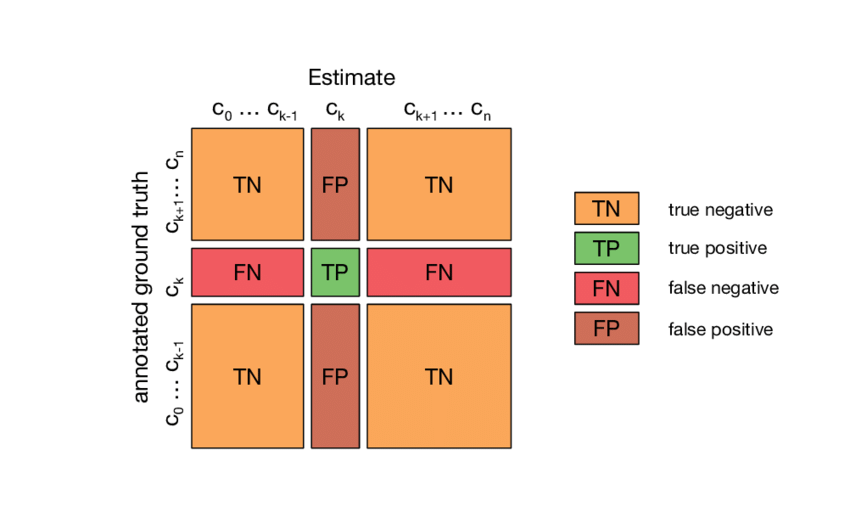
\includegraphics[scale=0.4]{Images/confusion_matrix.png}
    \caption{Confusion matrix for multiclass problem~\cite{ConfusionMatrix}.}
    \label{fig:confusionMatrix}
\end{figure}

\textbf{Accuracy}: Accuracy is the ratio of correctly classified samples to the total number of samples. It is calculated as:
\begin{equation}
    \text{Accuracy} = \frac{\sum_{i=1}^{m} TP_i + \sum_{i \neq j} TN_{ij}}{\sum_{i=1}^{m} (TP_i + FN_i + FP_i + TN_i)}
\end{equation}

\textbf{Precision}: Precision for a class $i$ measures the proportion of correctly predicted instances of class $i$ to the total instances predicted as class $i$. It is given by:
\begin{equation}
    \text{Precision}_i = \frac{TP_i}{TP_i + FP_i}
\end{equation}

\textbf{Recall}: Recall for a class $i$, also known as Sensitivity, measures the proportion of correctly predicted instances of class $i$ to all actual instances of class $i$. The formula is:
\begin{equation}
    \text{Recall}_i = \frac{TP_i}{TP_i + FN_i}
\end{equation}

\textbf{Macro-Averaged Precision and Recall}: To obtain a single performance metric across all classes, macro-averaging can also be used. This approach calculates the precision and recall for each class individually and then averages these values. Macro-averaging treats all classes equally, regardless of their size.

The macro-averaged precision is given by:
\begin{equation}
    \text{Macro Averaged Precision} = \frac{1}{m} \sum_{i=1}^{m} \text{Precision}_i
\end{equation}

The macro-averaged recall is given by:
\begin{equation}
    \text{Macro Averaged Recall} = \frac{1}{m} \sum_{i=1}^{m} \text{Recall}_i
\end{equation}

\textbf{F1 Score}: The F1 score for a class $i$ is the harmonic mean of precision and recall, providing a single metric that balances both concerns. It is calculated as:
\begin{equation}
\text{F1 Score}_i = 2 \times \frac{\text{Precision}_i \times \text{Recall}_i}{\text{Precision}_i + \text{Recall}_i}
\end{equation}
For multiclass problems, the average F1 score across all classes can be used:
\begin{equation}
\text{F1 Score (Macro)} = \frac{1}{m} \sum_{i=1}^{m} \text{F1 Score}_i
\end{equation}

\textbf{Receiver Operating Characteristic (ROC)}: The ROC curve is a graphical plot that illustrates the diagnostic ability of a binary classifier system as its discrimination threshold is varied. The curve is created by plotting the true positive rate (TPR) against the false positive rate (FPR) at various threshold settings. For multiclass classification, ROC curves can be plotted using a one-vs-rest approach, where each class is compared against all other classes.

\begin{figure}[H]
    \centering    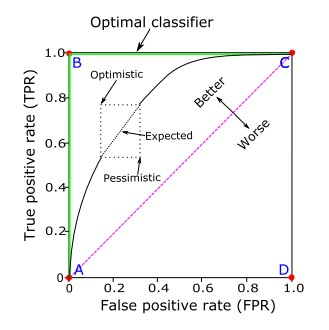
\includegraphics[scale=0.8]{Images/roc_curve.jpg}
    \caption{A basic ROC curve illustrating key points, along with the optimistic, pessimistic, and expected ROC segment~\cite{ClassificationMetrics}.}
    \label{fig:roc_curve}
\end{figure}


\textbf{Area Under the Curve (AUC)}: The AUC is a performance measurement for classification problems at various threshold settings. The AUC represents the degree or measure of separability; it tells how much the model is capable of distinguishing between classes. The AUC is calculated as the area under the Receiver Operating Characteristic (ROC) curve. The ROC curve is a plot of the true positive rate (TPR) against the false positive rate (FPR) at various threshold levels. For a multiclass problem, AUC is computed by considering each class versus the rest.

The AUC is given by:
\begin{equation}
    \text{AUC} = \int_{0}^{1} \text{TPR}(\text{FPR}^{-1}(x)) \, dx
\end{equation}

where:

\begin{equation}
    TPR = \frac{TP}{TP + FN}
\end{equation}

and:

\begin{equation}
    FPR = \frac{FP}{FP + TN}
\end{equation}

For multiclass problems, the AUC can be calculated using a one-vs-rest approach where the ROC curve is plotted for each class against all other classes, and then the average AUC is computed.

\textbf{Macro-Averaged AUC}: Similar to macro-averaging for precision and recall, the macro-averaged AUC is calculated by averaging the AUC values of each class.

The macro-averaged AUC is given by:
\begin{equation}
    \text{Macro Averaged AUC} = \frac{1}{m} \sum_{i=1}^{m} \text{AUC}_i
\end{equation}

\section{Saliency maps}

Saliency maps, used in these experiments, enable the visualization of pixels that had the most significant impact on the decision made by a convolutional neural network. This is achieved by creating a heat map or other graphical representation with dimensions equal to the analyzed image, where pixels with greater influence on the decision have higher values. Saliency maps provide deeper insight into the network's decision-making process, which can lead to the development of better network architectures. Additionally, they allow us to identify incorrectly made decisions by the network. Before the discovery of saliency maps, improving network architectures was limited to trial and error, which was highly unsatisfactory from a scientific point of view.

Two of the most popular methods for generating saliency maps are \textbf{\textit{Grad-CAM}} and \textbf{\textit{Grad-CAM++}}. \textit{Grad-CAM} (Gradient-weighted Class Activation Mapping) uses the gradients of any target concept, flowing into the final convolutional layer to produce a coarse localization map highlighting the important regions in the image for predicting the concept. \textit{Grad-CAM++} is an improved version that provides better localization and sharper visualizations by considering the positive partial derivatives of the gradients with respect to the feature maps. These methods have become widely used due to their effectiveness and ease of interpretation.

The image below demonstrates the application of \textit{Grad-CAM++} to understand the reason for prediction errors made by a convolutional neural network.

\begin{figure}[H]
    \centering    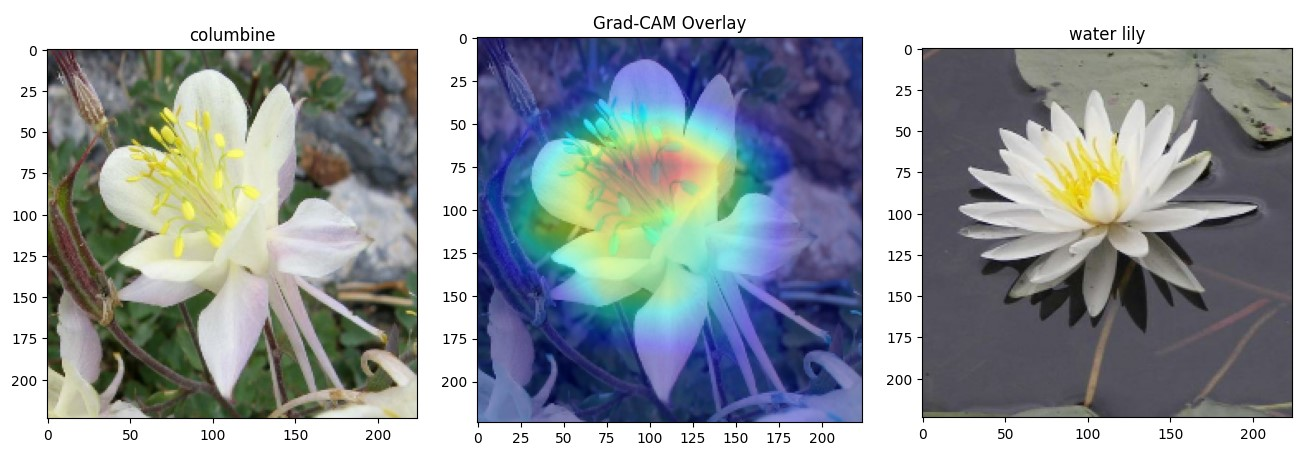
\includegraphics[scale=0.4]{Images/gradcam_mine_example.jpg}
    \caption{\textit{Grad-CAM++} Example.}
    \label{fig:gradcamMine}
\end{figure}

In the left image, we see the original flower (columbine) that was used for prediction. The middle image shows a \textit{Grad-CAM++} visualization overlay, highlighting the regions that the network focused on to make its prediction. The right image shows a sample from the class that the network predicted (water lily).


Using the \textit{Grad-CAM++} visualization, it is evident that the network heavily focused on the yellow part of the flower. Both the columbine and the water lily have prominent yellow sections, likely causing the network to misclassify the columbine as a water lily. Saliency maps, such as the \textit{Grad-CAM++} visualization, help us understand why such mistakes occur. This understanding enables us to refine and improve our model by adjusting the training data, augmenting features, or rethinking the network architecture to reduce similar errors in the future.